\begin{figure}[!ht]
\begin{center}
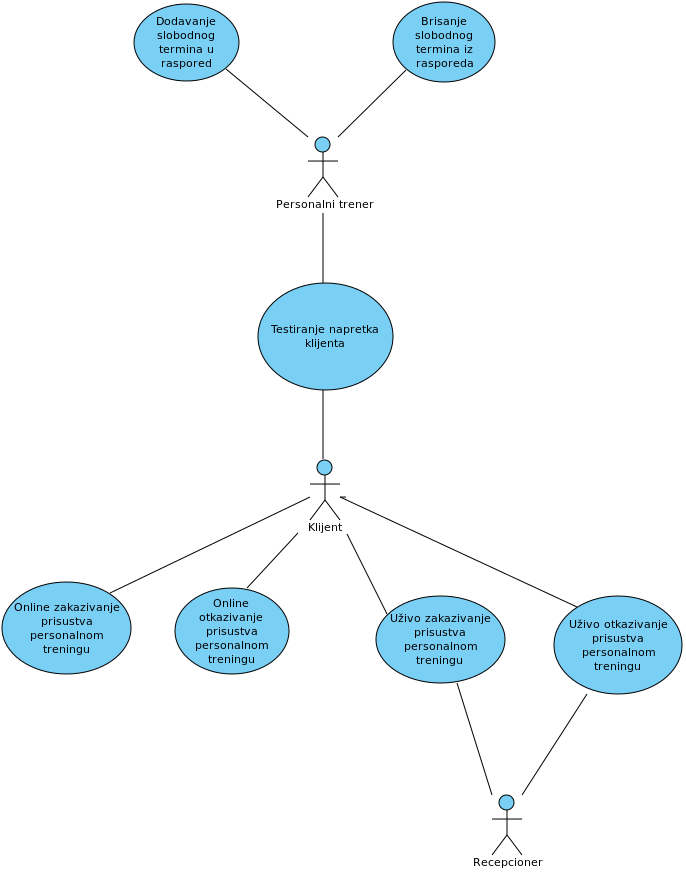
\includegraphics[scale=0.55]{sections/images/personalni_treninzi_slucajevi_upotrebe.png}
\end{center}
\caption{Dijagram slučajeva upotrebe za aktivnosti vezane za personalne treninge}
\label{fig:kontekst}
\end{figure}

\newpage

\subsubsection{Slučaj upotrebe: Dodavanje slobodnog termina u raspored}


\begin{longtable}{| p{.20\textwidth} | p{.80\textwidth} |} 
\hline
    Kratak opis &  Personalni trener vrši dodavanje slobodnog termina u svoj raspored treninga preko lične stranice na sistemu.\\ 
\hline    
    Učesnici &
    \begin{enumerate}
        \item Personalni trener - želi da doda novi slobodan termin u svoj raspored treninga
    \end{enumerate}\\
\hline
   Preduslovi & 
   \begin{enumerate}
        \item Personalni trener ima pristup internetu
        \item Personalni trener ima svoj nalog na sistemu
    \end{enumerate}\\
\hline  
    Postuslovi &
    \begin{enumerate}
        \item Termin je dodat i izmenjen je lični raspored personalnog trenera
    \end{enumerate}\\
\hline
    Osnovni tok & 
    \begin{enumerate}
        \item Personalni trener se prijavljuje na sistem
        \item Personalni trener odlazi na svoju stranicu na sistemu.
        \item Personalni trener pristupa delu stranice u kom se nalazi njegov raspored treninga.
        \item Personalni trener dodaje novu stavku u svoj raspored tako što unosi dan, sat početka i sat završetka treninga.
        \item Sistem čuva informaciju o izboru i ažurira lični raspored personalnog trenera.
    \end{enumerate}\\
\hline
    Alternativni tokovi & /\\
\hline
    Podtokovi & /\\
\hline
    Specijalni zahtevi & /\\
\hline
    Dodatne informacije & /\\
\hline
\caption{Dodavanje slobodnog termina u raspored} % needs to go inside longtable environment    
\end{longtable}





\subsubsection{Slučaj upotrebe: Brisanje slobodnog termina iz rasporeda}

\begin{longtable}{| p{.20\textwidth} | p{.80\textwidth} |} 
\hline
    Kratak opis & Personalni trener vrši brisanje slobodnog termina iz svog rasporeda. \\ 
\hline    
    Učesnici &
    \begin{enumerate}
    \item  Personalni trener - želi da doda ukloni slobodan termin iz svog rasporeda treninga. 
    \end{enumerate}\\
\hline
   Preduslovi & \begin{enumerate}
    \item Personalni trener ima pristup internetu
    \item Personalni trener ima svoj nalog na sistemu
    \item Personalni trener ima slobodne termine u svom rasporedu
    \end{enumerate} \\
\hline  
    Postuslovi & 
    \begin{enumerate}
    \item Termin je izbrisan i izmenjen je lični raspored personalnog trenera
    \end{enumerate}\\
\hline
    Osnovni tok & 
    \begin{enumerate}
    \item Personalni trener se prijavljuje na sistem
    \item Personalni trener odlazi na svoju stranicu na sistemu
    \item Personalni trener pristupa delu stranice u kom se nalazi njegov raspored treninga
    \item Personalni trener briše slobodan termin tako što bira opciju 'Ukloni' koja se nalazi pored datog slobodnog termina
    \item Sistem čuva informaciju o brisanju i ažurira lični raspored personalnog trenera
    \end{enumerate}\\
\hline
    Alternativni tokovi & /\\
\hline
    Podtokovi & /\\
\hline
    Specijalni zahtevi & /\\
\hline
    Dodatne informacije & /\\
\hline
\caption{Brisanje slobodnog termina iz rasporeda}
\end{longtable}



\subsubsection{Slučaj upotrebe: Online zakazivanje prisustva personalnom treningu}



\begin{longtable}{| p{.20\textwidth} | p{.80\textwidth} |} 
\hline
    Kratak opis & Klijent zakazuje prisustvo personalnom treningu tako što bira personalnog trenera na čiji trening želi da ode, a zatim i jedan od ponuđenih slobodnih termina iz rasporeda tog trenera. \\ 
\hline    
    Učesnici & 
    \begin{enumerate}
    \item  Klijent - želi da zakaže prisustvo personalnom treningu
    \end{enumerate}\\
\hline
   Preduslovi & 
   \begin{enumerate}
    \item Klijent ima pristup internetu
    \item Klijent je registrovan
   \end{enumerate} \\
\hline  
    Postuslovi & 
    \begin{enumerate}
    \item Izmenjen je lični raspored personalnog trenera
    \item Izmenjen je lični raspored klijenta
   \end{enumerate} \\
\hline
    Osnovni tok &
    \begin{enumerate}
   \item Klijent se prijavljuje na sistem
    \item Klijent odlazi na stranicu personalnog trenera kod koga želi da trenira
    \item Klijent bira jedan od ponuđenih slobodnih termina iz rasporeda tog trenera tako što klikne na opciju 'Zakaži' koja se nalazi pored svakog slobodnog termina
    \item Sistem ažurira lične rasporede personalnog trenera (tako što unosi ime i prezime klijenta) i klijenta (tako što unosi dan i sat treninga i ime i prezime trenera)
    \item Sistem obaveštava klijenta da je uspešno zakazano prisustvo treningu
    \item Sistem obaveštava personalnog trenera da je zakazano prisustvo jednom njegovom treningu
   \end{enumerate} \\
\hline
    Alternativni tokovi & 
    \begin{itemize}
    \item[A1] Neispravni podaci u prijavi. Ukoliko klijent prilikom prijave na sistem u koraku 1 unese pogrešne podatke, sistem ga obaveštava o tome. Slučaj upotrebe se nastavlja u koraku 1.
    \item[A3.1] Nema slobodnih termina. Ukoliko u koraku 3. nema slobodnih termina u rasporedu treninga odabranog trenera, klijent može da bira drugog trenera. Slučaj upotrebe se vraća na korak 2.
    \item[A3.2] Klijentu ne odgovaraju slobodni termini. Ukoliko u koraku 3. ima slobodnih termina u rasporedu treninga odabranog trenera, ali klijentu ne odgovara nijedan, klijent bira drugog trenera. Slučaj upotrebe se vraća na korak 2.
    \item[A3.3] Klijentu ne odgovara nijedan slobodan termin nijednog personalnog trenera. Ukoliko ponavljanjem koraka 2. i 3. klijent ne pronađe termin koji mu odgovara, onda neće zakazati prisustvo nijednom treningu te nedelje. Slučaj upotrebe se završava.
   \end{itemize} \\
\hline
    Podtokovi & /\\
\hline
    Specijalni zahtevi & /\\
\hline
    Dodatne informacije & / \\
\hline
\caption{ Online zakazivanje prisustva personalnom treningu}
\end{longtable}


\newpage
\begin{figure}[!ht]
\begin{center}
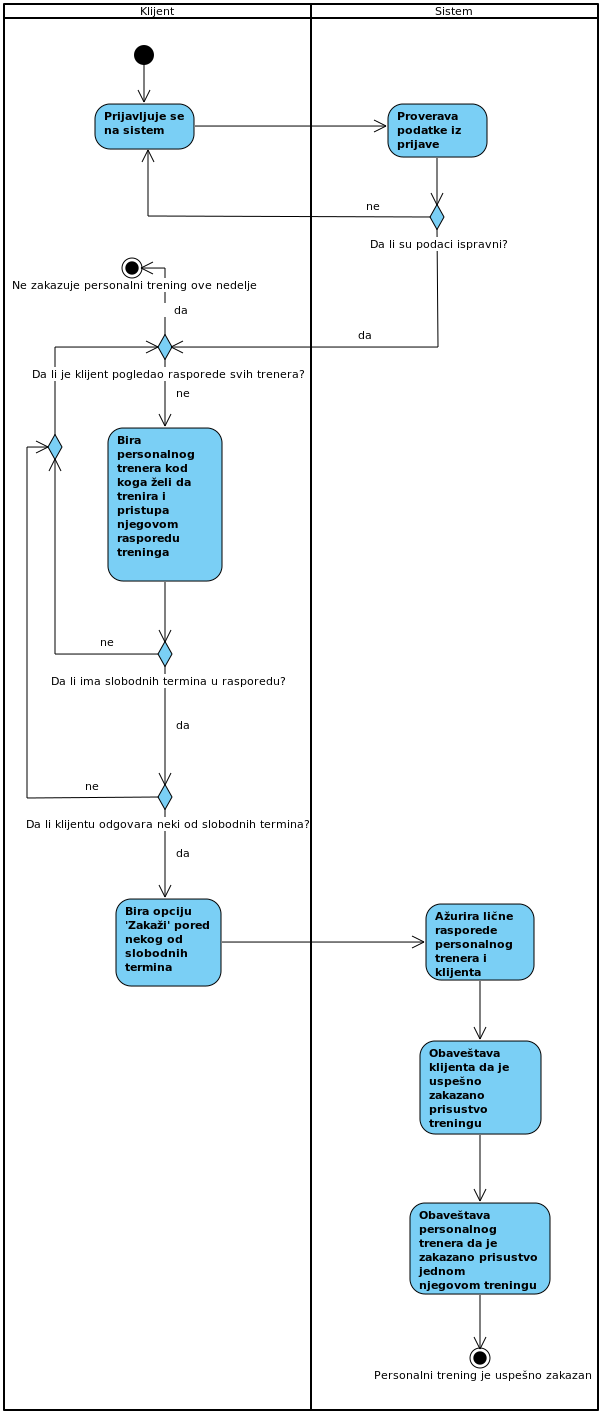
\includegraphics[scale=0.38]{sections/images/dijagram-aktivnosti-personalni-online-zakazivanje-prisustva.png}
\end{center}
\caption{Dijagram aktivnosti online zakazivanja prisustva personalnom treningu}
\label{fig:kontekst}
\end{figure}



\subsubsection{Slučaj upotrebe: Online otkazivanje prisustva personalnom treningu}


\begin{longtable}{| p{.20\textwidth} | p{.80\textwidth} |} 
\hline
    Kratak opis & Klijent otakazuje prisustvo prethodno prijavljenom personalnom treningu \\ 
\hline    
    Učesnici &  
    \begin{enumerate}
    \item Klijent - želi da otkaže prisustvo personalnom treningu
    \end{enumerate}\\
\hline
   Preduslovi & 
   \begin{enumerate}
    \item Klijent ima pristup internetu
    \item Klijent je registrovan
    \item Klijent ima prijavljeno prisustvo bar jednom personalnom treningu
   \end{enumerate}\\
\hline  
    Postuslovi & 
    \begin{enumerate}
    \item Izmenjen je lični raspored personalnog trenera
    \item Izmenjen je lični raspored klijenta
   \end{enumerate} \\
\hline
    Osnovni tok & 
    \begin{enumerate}
    \item Klijent se prijavljuje na sistem
    \item Klijent odlazi na stranicu koja sadrži njegov lični raspored
    \item Klijent bira opciju 'Otkaži' pored onog treninga kom više ne želi da prisustvuje
    \item Sistem paralelno ažurira lični raspored klijenta (tako što iz njega uklanja taj trening) i lični raspored personalnog trenera koji drži taj trening (tako što uklanja ime i prezime korisnika čime dati termin postaje slobodan)
    \item Sistem obaveštava klijenta da je uspešno otkazano prisustvo treningu
   \end{enumerate}\\
\hline
    Alternativni tokovi & /\\
\hline
    Podtokovi & /\\
\hline
    Specijalni zahtevi & /\\
\hline
    Dodatne informacije & /\\
\hline
\caption{Online otkazivanje prisustva personalnom treningu}
\end{longtable}




\subsubsection{Slučaj upotrebe: Uživo zakazivanje prisustva personalnom treningu}

\begin{longtable}{| p{.20\textwidth} | p{.80\textwidth} |} 
\hline
    Kratak opis & Klijent zakazuje prisustvo personalnom treningu na recepciji. \\ 
\hline    
    Učesnici & 
    \begin{enumerate}
    \item Klijent - želi da zakaže prisustvo personalnom treningu
    \item Recepcioner - prijavljuje klijenta za željeni trening
   \end{enumerate}\\
\hline
   Preduslovi & \begin{enumerate}
    \item Sistem je u funkciji.
    \item Klijent je registrovan.
    \item Klijent razgovora uživo sa recepcionarem.
   \end{enumerate} \\
\hline  
    Postuslovi & \begin{enumerate}
    \item Klijent je dobio potvrdu da je njegov trening zakazan.
    \item Izmenjen je lični raspored personalnog trenera
    \item Izmenjen je lični raspored klijenta
   \end{enumerate} \\
\hline
    Osnovni tok & 
    \begin{enumerate}
    \item Klijent dolazi na recepciju sportskog centra.
    \item Recepcionar traži od korisnika da mu da člansku kartu ili username
    \item Klijent daje recepcionaru svoju člansku kartu ili username
    \item Recepcionar se povezuje na deo sistema preko kojeg je u mogućnosti da ažurira korisnički nalog.
    \item Klijent bira trenera na čiji trening želi da se prijavi
    \item Recepcioner proverava raspored tog trenera i govori klijentu slobodne termine
    \item Klijent bira termin koji mu odgovara
    \item Recepcioner unosi informacije u sistem
    \item Sistem paralelno ažurira lične rasporede klijenta i trenera
    \item Sistem obaveštava recepcionera da je zakazano prisustvo treningu
    \item Recepcioner obaveštava klijenta da je zakazano prisustvo treningu
    \item Sistem obaveštava trenera da je zakazano prisustvo jednom njegovom treningu
   \end{enumerate}\\
\hline
    Alternativni tokovi & 
    \begin{itemize}
    \item[A6.1] Nema slobodnih termina. Ukoliko u koraku 6. nema slobodnih termina u rasporedu treninga odabranog trenera, recepcioner obaveštava korisnika o tome i govori mu da izabere drugog trenera. Slučaj upotrebe se vraća na korak 5.
    \item[A6.2] Klijentu ne odgovaraju slobodni termini. Ukoliko u koraku 6. ima slobodnih termina u rasporedu treninga odabranog trenera, ali klijentu ne odgovara nijedan, klijent govori recepcioneru da mu ne odgovara nijedan ponuđeni termin i da želi da izabere drugog trenera. Slučaj upotrebe se vraća na korak 5.
    \item[A6.3] Klijentu ne odgovara nijedan slobodan termin nijednog personalnog trenera. Ukoliko ponavljanjem koraka 5. i 6. klijent ne pronađe termin koji mu odgovara, onda neće zakazati prisustvo nijednom treningu te nedelje. Slučaj upotrebe se završava.
   \end{itemize}\\
\hline
    Podtokovi & /\\
\hline
    Specijalni zahtevi & /\\
\hline
    Dodatne informacije & /\\
\hline
\caption{Uživo zakazivanje prisustva personalnom treningu}
\end{longtable}


    
   



\subsubsection{Slučaj upotrebe: Uživo otkazivanje prisustva personalnom treningu}

\begin{longtable}{| p{.20\textwidth} | p{.80\textwidth} |} 
\hline
    Kratak opis & Klijent otkazuje prisustvo prethodno prijavljenom personalnom treningu na recepciji. \\ 
\hline    
    Učesnici &
    \begin{enumerate}
    \item Klijent - želi da otkaže prisustvo personalnom treningu
    \item Recepcioner - odjavljuje klijenta sa odabranog treninga
   \end{enumerate}\\
\hline
   Preduslovi & \begin{enumerate}
    \item Sistem je u funkciji.
    \item Klijent je registrovan.
    \item Klijent razgovora uživo sa recepcionarem.
    \item Klijent ima prijavljeno prisustvo bar jednom personalnom treningu
   \end{enumerate} \\
\hline  
    Postuslovi &
    \begin{enumerate}
    \item Klijent je dobio potvrdu da je otkazano njegovo prisustvo treningu
    \item Izmenjen je lični raspored personalnog trenera
    \item Izmenjen je lični raspored klijenta
   \end{enumerate}\\
\hline
    Osnovni tok & 
    \begin{enumerate}
    \item Klijent dolazi na recepciju sportskog centra.
    \item Recepcionar traži od korisnika da mu da člansku kartu ili username
    \item Klijent daje recepcionaru svoju člansku kartu ili username
    \item Recepcionar se povezuje na deo sistema preko kojeg je u mogućnosti da ažurira korisnički nalog.
    \item Klijent mu govori koji je to trening kom ne želi da prisustvuje - daje mu ime i prezime trenera i termin treninga
    \item Recepcioner u rasporedu klijenta pronalazi taj trening i bira opciju 'Otkaži' 
    \item Sistem paralelno ažurira lične rasporede klijenta i trenera
    \item Sistem obaveštava recepcionera da je otkazano prisustvo treningu
    \item Recepcioner obaveštava klijenta da je otkazano prisustvo treningu
    \item Sistem obaveštava trenera da je otkazano prisustvo jednom njegovom treningu i da je taj termin ponovo slobodan
   \end{enumerate}\\
\hline
    Alternativni tokovi & /\\
\hline
    Podtokovi & /\\
\hline
    Specijalni zahtevi & /\\
\hline
    Dodatne informacije & /\\
\hline
\caption{Uživo otkazivanje prisustva personalnom treningu}
\end{longtable}


 